\begin{tikzpicture}[
  ->, % makes the edges directed
  >=stealth', % makes the arrow heads bold
  node distance=3cm, % specifies the minimum distance between two nodes. Change if necessary.
  every state/.style={thick, fill=gray!10}, % sets the properties for each ’state’ node
  initial text=$ $, % sets the text that appears on the start arrow
]
\node[state, initial right] (start) {$v_6$};
\node[state, left of=start] (s) {$v_7$};
\node[state, left of=s, accepting] (pes-filipes) {$v_8$};
\node[state, below of=s] (k) {$v_9$};
\node[state, left of=k, accepting] (pejsek) {$v_{10}$};
\node[state, below of=pejsek, accepting] (maxipes-fik) {$v_{11}$};

\node[left of=pes-filipes] (pes-filipes-drawing) {\scalebox{-1}[1]{
\includegraphics[height=2cm,trim={0 4.75cm 0 0},clip]{figures/pes-filipes}}};
\node[left of=pejsek] (pejsek-drawing) {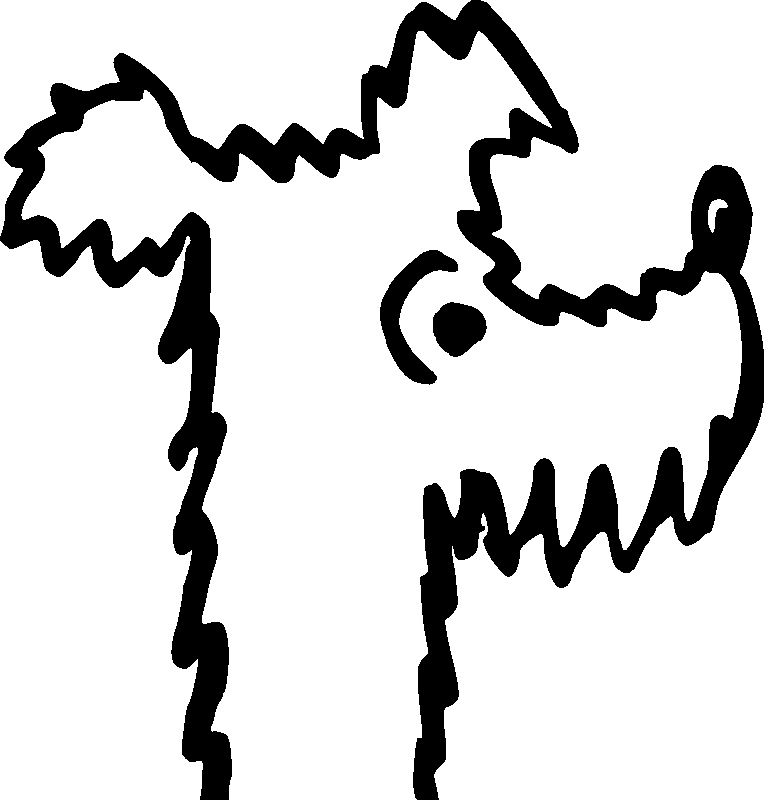
\includegraphics[height=2cm]{figures/pejsek}};
\node[left of=maxipes-fik] (maxipes-fik-drawing) {
\includegraphics[height=2cm]{figures/maxipes-fik}};

\draw (start) edge node[above]{s} (s);
\draw (s) edge node[above]{pes\textvisiblespace filipe} (pes-filipes);
\draw (pes-filipes) edge (pes-filipes-drawing);
\draw (start) edge node[above, rotate=45]{k} (k);
\draw (k) edge node[above]{pejse} (pejsek);
\draw (pejsek) edge (pejsek-drawing);
\draw (k) edge node[above, rotate=45]{maxipes\textvisiblespace fí} (maxipes-fik);
\draw (maxipes-fik) edge (maxipes-fik-drawing);
\end{tikzpicture}